%%%%%%%%%%%%%%%%%%%%%%%%%%%%%%%%%%%%%%%%%%%%%%%%%%%%%%%%%%%%%%%%%%%%%%%%%%%%
% AGUJournalTemplate.tex: this template file is for articles formatted with LaTeX
%
% This file includes commands and instructions
% given in the order necessary to produce a final output that will
% satisfy AGU requirements, including customized APA reference formatting.
%
% You may copy this file and give it your
% article name, and enter your text.
% guidelines and troubleshooting are here: 

%% To submit your paper:
%% NOTES:
% DON'T USE SUBFIGURES!!!!

\documentclass[12pts,draft]{AR_analysis_}
% \usepackage{hyperref} % creates a hyperlink to the figure referenced
\usepackage{url} %this package should fix any errors with URLs in refs.
\usepackage{lineno}
%for better track changes. finalnew option will compile document with changes incorporated.
\usepackage[inline]{trackchanges}
\usepackage{soul}
\usepackage{float}  % Required for the [H] option
\usepackage{graphicx} % for my graphics
\usepackage{xcolor} % for my graphics
\usepackage{textcomp} % removes warning in gensymb
\usepackage{gensymb} % for basic symbols like degree
\usepackage{mathtools}
\usepackage{amsmath}
\usepackage{tabularx}
\usepackage{booktabs}
%\usepackage{subcaption}

\usepackage{makecell}
\usepackage{array}

\newcolumntype{R}[1]{>{\raggedleft\arraybackslash}m{#1}}

% Bottom four packages from matplotlib -> LaTeX 
% Tutorial
% https://blog.timodenk.com/exporting-matplotlib-plots-to-latex/
\usepackage{tikz}
\usepackage{tikz-cd}
\usepackage{pgfplots}
\pgfplotsset{compat=1.14}

\linenumbers

%%%%%%%
% As of 2018 we recommend use of the TrackChanges package to mark revisions.
% The trackchanges package adds five new LaTeX commands:
%
%  \note[editor]{The note}
%  \annote[editor]{Text to annotate}{The note}
%  \add[editor]{Text to add}
%  \remove[editor]{Text to remove}
%  \change[editor]{Text to remove}{Text to add}
%
% complete documentation is here: http://trackchanges.sourceforge.net/
%%%%%%%

\draftfalse

%% Enter journal name below.
%% Choose from this list of Journals:
%
% JGR: Atmospheres
% JGR: Biogeosciences
% JGR: Earth Surface
% JGR: Oceans
% JGR: Planets
% JGR: Solid Earth
% JGR: Space Physics
% Global Biogeochemical Cycles
% Geophysical Research Letters
% Paleoceanography and Paleoclimatology
% Radio Science
% Reviews of Geophysics
% Tectonics
% Space Weather
% Water Resources Research
% Geochemistry, Geophysics, Geosystems
% Journal of Advances in Modeling Earth Systems (JAMES)
% Earth's Future
% Earth and Space Science
% Geohealth
%
% ie, \journalname{Water Resources Research}

\journalname{Geophysical Research Letters}

\begin{document}

%%%%%%%%%%%%%%%%%%%%%%%%%%%%%%%%%%%%%%%%%%%%%%%
%  TITLE
%
% (A title should be specific, informative, and brief. Use
% abbreviations only if they are defined in the abstract. Titles that
% start with general keywords then specific terms are optimized in
% searches)
%
%%%%%%%%%%%%%%%%%%%%%%%%%%%%%%%%%%%%%%%%%%%%%%%

\title{Influence of Atmospheric Rivers on Alaskan River Ice}

%%%%%%%%%%%%%%%%%%%%%%%%%%%%%%%%%%%%%%%%%%%%%%%
%
%  AUTHORS AND AFFILIATIONS
%
%%%%%%%%%%%%%%%%%%%%%%%%%%%%%%%%%%%%%%%%%%%%%%%

% Authors are individuals who have significantly contributed to the
% research and preparation of the article. Group authors are allowed, if
% each author in the group is separately identified in an appendix.)

% List authors by first name or initial followed by last name and
% separated by commas. Use \affil{} to number affiliations, and
% \thanks{} for author notes.
% Additional author notes should be indicated with \thanks{} (for
% example, for current addresses).

\authors{Russ Limber\affil{1, 2}, Elias C. Massoud\affil{2}, 
Jitendra Kumar\affil{2}, Bin Guan\affil{3}, Forrest M. Hoffman\affil{2}}
\affiliation{1}{The University of Tennessee}
\affiliation{2}{Oak Ridge National Laboratory}
\affiliation{3}{University of California, Los Angeles}

%(repeat as many times as is necessary)

% Corresponding author mailing address and e-mail address:

% (include name and email addresses of the corresponding author.  More
% than one corresponding author is allowed in this LaTeX file and for
% publication; but only one corresponding author is allowed in our
% editorial system.)

% Example: \correspondingauthor{First and Last Name}{email@address.edu}
\correspondingauthor{Russ Limber}{r62@ornl.gov}


%%%%%%%%%%%%%%%%%%%%%%%%%%%%%%%%%%%%%%%%%%%%%%%
% KEY POINTS
%%%%%%%%%%%%%%%%%%%%%%%%%%%%%%%%%%%%%%%%%%%%%%%
%  List up to three key points (at least one is required)
%  Key Points summarize the main points and conclusions of the article
%  Each must be 140 characters or fewer with no special characters 
% or punctuation and must be complete sentences

% Example:
% \begin{keypoints}
% \item	List up to three key points (at least one is required)
% \item	Key Points summarize the main points and conclusions of the article
% \item	Each must be 140 characters or fewer with no special 
	% characters or punctuation and must be complete sentences
% \end{keypoints}

% These are all under 140 characters
\begin{keypoints}

\item Atmospheric Rivers (ARs) generally lead to a week-long persistent 
	increase in daily temperature over Interior Alaska (AK)

\item In AK, ARs account for 36\% of total precipitation, 57\% of extreme 
	precipitation and explain 48\% of interannual variability of precipitation

\item AR events during the coldest months prolong the annual breakup date of 
	river ice, while ARs closer to the breakup date have less impact.

\end{keypoints}

%%%%%%%%%%%%%%%%%%%%%%%%%%%%%%%%%%%%%%%%%%%%%%%
%
%  ABSTRACT and PLAIN LANGUAGE SUMMARY
%
% A good Abstract will begin with a short description of the problem
% being addressed, briefly describe the new data or analyses, then
% briefly states the main conclusion(s) and how they are supported and
% uncertainties.

% The Plain Language Summary should be written for a broad audience,
% including journalists and the science-interested public, that will not have 
% a background in your field.
%
% A Plain Language Summary is required in GRL, JGR: Planets, JGR: Biogeosciences,
% JGR: Oceans, G-Cubed, Reviews of Geophysics, and JAMES.
% see http://sharingscience.agu.org/creating-plain-language-summary/)
%
%%%%%%%%%%%%%%%%%%%%%%%%%%%%%%%%%%%%%%%%%%%%%%%

%% \begin{abstract} starts the second page
%% The Abstract should be a single paragraph of fewer than 250 words
%% (for Geophysical Research Letters, under 150 words). 

\begin{abstract}
	
	Atmospheric rivers (ARs) transport vast amounts of moisture 
	from low to high latitude regions. One region particularly 
	impacted by ARs is Interior Alaska (AK). We analyze the impact 
	of ARs on the annual river ice breakup date for 25 locations 
	in AK. We investigate the AR-driven rise in local temperatures 
	and explore the relationship between ARs and precipitation, 
	including extremes and interannual variability. We found that 
	the increase in local temperatures after an AR event can last 
	for as long as one week. Our results show that ARs account 
	for 36\% of total precipitation, explain 48\% of precipitation 
	variability, and make up 57\% of extreme precipitation events. 
	Calculating the heat transfer between ARs and river ice, we 
	conclude that heavy precipitation events  (HPEs) during the 
	coldest period of the year prolong river ice breakup dates, 
	while HPEs occurring close to the breakup date have little 
	impact on breakup timing. 

\end{abstract}

% The PLS should be a single paragraph no more than 200 words long.

\section*{Plain language summary}

	Atmospheric Rivers (ARs) are large storm systems originating in
	tropical regions capable of depositing large amounts of
	precipitation as far north as the Arctic. 
	Using river ice breakup data recorded throughout Interior
	Alaska (AK) we set out to find whether there exists a link between
	ARs and annual river ice breakup timing. We determined that 
	daily temperature increases can last  up to
	one week after an AR event. We also found that ARs
	account for 36\% of total annual precipitation from 1980 to 2023, 
	explain 48\% of the variability of precipitation, and make up 57\% 
	of extreme precipitation events. We then
	calculated the total heat transfer between precipitation and river
	ice and found that heavy precipitation events (HPEs),
	from both local precipitation and ARs, that occur relatively close to
	river ice breakup dates, have little correlation to the breakup
	date. However, HPEs that occur during the coldest period of the
	year (typically late December to early-February) are strongly inversely
	correlated with river ice breakup timing, and therefore prolong
	the breakup date.

%%%%%%%%%%%%%%%%%%%%%%%%%%%%%%%%%%%%%%%%%%%%%%%
%
%  BODY TEXT
%
%%%%%%%%%%%%%%%%%%%%%%%%%%%%%%%%%%%%%%%%%%%%%%%

%%% Suggested section heads:
% \section{Introduction}
%
% The main text should start with an introduction. Except for short
% manuscripts (such as comments and replies), the text should be divided
% into sections, each with its own heading.

% Headings should be sentence fragments and do not begin with a
% lowercase letter or number. Examples of good headings are:

% \section{Materials and Methods}
% Here is text on Materials and Methods.
%
% \subsection{A descriptive heading about methods}
% More about Methods.
%
% \section{Data} (Or section title might be a descriptive heading about data)
%
% \section{Results} (Or section title might be a descriptive heading about the
% results)
%
% \section{Conclusions}



\section{Introduction}

Atmospheric rivers (ARs) are narrow corridors of intense water vapor
transport that significantly influence hydrologic events, transporting
most of the water vapor outside of the Tropics \cite{NOAA_AR_summary}.
It is estimated that ARs are responsible for as much as 90\% of poleward
water vapor transport at midlatitudes \cite{other_alg}. ARs contribute to
extreme precipitation events across various regions worldwide 
\cite{Espinoza2018, Massoud2019}, including
Western North America \cite{Dettinger2004, Neiman2008, Guan2010,
ARs_flood_WA_State, ARs_flood_Russian_River_CA, Ralph2013, ARs_CA}
Europe \cite{Lavers2013, ARs_impact_Norway}, the Middle East \cite{massoud2020, 
Lashkari2020,  Esfandiari2024}, and Western South America
\cite{ARs_impact_SA}. In recent years, the impacts of ARs on the cryosphere
such as Greenland \cite{Mattingly2018} and Antarctica \cite{Gorodetskaya2014, 
Wille2021}, have been more extensively analyzed. 

In recent years, a growing number of works 
investigating the relationship between ARs and 
high latitude regions has been underway. Evidence shows that between
1981 and 2020, higher atmospheric moisture content was significantly correlated
with lower sea ice coverage over almost the entire Arctic Ocean
\cite{ARs_lead_to_sea_ice_loss}. For those same years, another analysis
found that 100\% of extreme temperature events in the Arctic (above 0
$\degree C$) coincide with the presence of ARs \cite{Ma2023}. Analyses have noted
a relationship between heavy AR activity and sea ice loss, caused by
increased rainfall from moisture originating in lower latitudes
\cite{Zhang2023, maclennan_contribution_2022}. However Arctic systems
are complicated, as the intense moisture transport within ARs can also
result in heavy snowfall events, thus contributing to the accumulation
of snowpack, especially in mountainous regions \cite{Saavedra2020,
Guan2010}. Under the right conditions, this relationship has been found
to actually increase the mass balance of glaciers \cite{Little2019}.
Understanding the role of ARs in the cryosphere is essential for
assessing their broader impact on regional water resources and glacier
dynamics in a changing climate. 

While a number of works have explored
the relationship between ARs and sea ice, glaciers, or ice sheets, 
to our knowledge there has
been no analysis that investigates the relationship between ARs and Arctic
river ice. Many works have used physics based processes
to model the annual breakup timing and conditions of Arctic river ice
\cite{Paily, ashton1986river, Prowse_Bonsal_Duguay_Lacroix_2007,
jasek1998, shen_newest}. Through such studies, it is recognized that an 
increase in precipitation leading to an increase in
streamflow alters the hydraulics surrounding river ice breakup timing, 
potentially accelerating mechanical breakup events \cite{ashton1986river}.
It has also been proposed that increased snow pack as a result of increased 
precipitation, contributes to breakup severity \cite{Prowes2002}. Using 
breakup records throughout Interior Alaska (AK) from the Alaska 
Pacific River Forecast Center Database
(the same breakup records used in this analysis) \citeA{Bieniek2011} determined 
that winter precipitation plays a relatively minor role in impacting the 
breakup timing of river ice and if anything accelerates the breakup timing as a 
result of increased streamflow. They go on to say that 
increased storm activity in the spring leads to increased surface air 
temperature, leading to earlier breakup dates \cite{Bieniek2011}. However, 
their analysis used only 4 sites (as opposed to the 25 used in this analysis) 
and aggregated precipitation seasonally without accounting for the interaction 
between winter precipitation and temperature that occurs at a finer temporal
resolution. Our analysis sets out to answer the following questions: 
1.) Since ARs have been known to impact Arctic systems by increasing 
temperatures, is there a change in
air temperature in different regions of AK corresponding to the 
presence of ARs?
2.) How do ARs contribute to precipitation throughout AK, 
considering how ARs impact total annual precipitation, interannual 
variability, and extreme events?
3.) How do ARs impact the timing of river ice breakup, does the presence 
of ARs accelerate or prolong the timing of river ice breakup?

\section{Data}

\subsection{AR Catalog}

Similar to previous studies, we define ARs using integrated vapor
transport (IVT) values constructed from 6-hourly values of 3‐D wind and
water vapor at eight pressure levels between 300 and 1,000
mb from the National Center for Environmental Protection (NCEP) 
reanalysis data product \cite{NCEP_NCAR_reanalysis}. 
AR detection is based on version3 of the tARget algorithm
\cite{Guan_Waliser2019, bin2022}.
The IVT values are calculated at the original
resolution from the NCEP
meteorological inputs \cite{NCEP_reanalysis}.
\citeA{alg_for_detecting_AR_moisture_fluxes} developed a global
AR detection algorithm, which was updated and validated later with in
situ and dropsonde data \cite{bin2022}. This algorithm is employed for
our study, which is based on a combination of the IVT magnitude,
direction, and geometry characteristics, to objectively identify ARs.
Contiguous regions of enhanced IVT transport are first identified from
magnitude thresholding (i.e., grid cells with IVT above the seasonally
and locally dependent $85^{th}$ percentile, or $100\frac{kg}{m*s}$, 
whichever is greater) and further filtered
using directional and geometry criteria requirements. Although the 
$100\frac{kg}{m*s}$ threshold is applied globally, it is intended for 
dry (including polar) regions since in other regions the 85th percentile 
is already larger than $100\frac{kg}{m*s}$. The detection
algorithm was applied to NCEP in its native resolution of $2.5 \degree$.
This detection algorithm had over 90\% agreement in detecting AR
landfall dates when compared with other AR detection methods, for Western
North America \cite{Neiman2008}, the United Kingdom \cite{Lavers2011}, 
and East Antarctica \cite{Gorodetskaya2014}. 

\subsection{Daymet Daily Surface Weather and Climatological Summaries}

Precipitation and daily
minimum and maximum temperatures ($T_{\text{min}}$ and $T_{\text{max}}$ respectively) 
from Oak Ridge National
Laboratory's Daymet $1kmx1km$ daily product were used, via the
Distributed Active Archive Center \cite{daymet}. Daymet precipitation, 
$T_{\text{min}}$ and $T_{\text{max}}$, were used in our analysis as they
have a strong agreement with NCEP temperature outputs for our 
region of interest
Figure \ref{fig:concatenated_maps_precip_temp_plot}C. Additionally, 
because Daymet is derived directly from in situ instruments 
and meteorological stations, it represents a robust 
dataset for precipitation and temperature predictions across North
America \cite{daymet2021}. This dataset has been a standard for validation 
among several analyses related to arctic regions \cite{Diro2019, 
Akinsanola2024}. The annual mean precipitation and 
temperature for the year 2021 over the AK region are shown in Figure 
\ref{fig:concatenated_maps_precip_temp_plot}AB, and 
Figure \ref{fig:concatenated_maps_precip_temp_plot}C 
shows the temperature profiles, precipitation and AR trends
for one of those location over one year (Crooked 
Creek at the Kuskokwim River in 2021). 

\begin{figure}
\centering
\includegraphics[width=1.0\textwidth]{./images/maps_and_time_series.png}
	\caption{top row: (left) map showing summated precipitation for the
	year 2021; (right) map of average temperature for 2021. bottom row:
	One of the 25 locations (Crooked Creek on the Kuskokwim
	River) for the year 2021. Yellow, orange, red represent the
	temperature profiles (fill plot of $T_{\text{min}}$ -
	$T_{\text{max}}$) from NCEP
	temperature data at 850, 925 and 1000mb respectively. Light
	green represents the Daymet temperature profile. Dark blue shows
	modeled precipitation from Daymet while the light blue stem
	plots depict AR events. The vertical purple dashed line shows the breakup
	date for the Kuskokwim River in 2021 for Crooked Creek.}
\label{fig:concatenated_maps_precip_temp_plot} 
\end{figure}

\subsection{River ice breakup records}

River ice breakup dates 
were obtained from the Alaska Pacific River Forecast Center database.
While exact coordinates were unavailable, locations 
were estimated based on proximity to weather stations and airports, to 
maintain spatial consistency with inputs used in Daymet’s meteorological 
models. There were 25 locations (shown in Figure 
\ref{fig:concatenated_maps_precip_temp_plot}) identified as 
having at least 35 breakup 
records between 1980 and 2023 (the current temporal availability of 
Daymet), although breakup records go as far back as 1896 for some 
locations. The 35 breakup records threshold was used because it 
allowed for the greatest 
number of locations with the most complete time series 
necessary for statistical analysis. There is always one breakup 
date per year, but not every year has a recorded date, so some 
years are represented as empty values in the dataset. On average, 
recorded break up dates range from mid March to late 
June. This dataset has been used in other analyses such as 
\cite{murphy2022, Brown2018, Bieniek2011}. As an example, 
the breakup date for Crooked Creek 
at the Kuskokwim River in 2021 occurred in early May and
is depicted in Figure 
\ref{fig:concatenated_maps_precip_temp_plot}C with a 
vertical purple dashed line.



\section{Methods}

To assess the influence of ARs on local temperature, we analyze 
the relationship between the presence of an AR and the temperature 
change at a specific location. The presence of an AR is represented 
numerically as a binary value indicating whether or not an AR is 
active on a particular date. We then estimate how many days this 
change in temperature lasts. To do this, we used a
varying temporal window combined with a pairwise t-test. In other 
words, for each
AR occurrence in the dataset, a lookback window and forecast 
window each equal to \emph{n}
days in length was created before and after the AR date, respectively,
whereby: $ n \in \{1, 2, 3, \ldots, 14\}$.
For values of \emph{n} greater than one day the mean was 
taken within each window
for $T_{\text{min}}$ and $T_{\text{max}}$. These aggregated 
temperatures were then
calculated over all locations. Aggregated temperature pairs 
were assessed using a one tailed pairwise t-test to check
whether ARs increased the local temperature over period of 
time \emph{n} $(\alpha =
0.05)$. 

We then explored how ARs contribute to precipitation, by
separating AR-based precipitation from the total amount. We 
then used the Wilcoxon rank-sum test \cite{Rey2011} to test 
the hypothesis 
that AR events tend to produce more precipitation than other
precipitation events. We opted to use a non-parametric 
test (Wilcoxon rank-sum test) 
because the distributions of precipitation were shown to
not be normally distributed after log transformation using the
Shapiro-Wilks test, \cite{shapiro_wilk_test}. We also estimated
the interannual variability of precipitation that ARs account for by
conducting a univariate ordinary least squares regression (OLS). 
For extremes, we extracted the top 5\% of precipitation events and determined 
what fraction of those events are associated with ARs. 

To determine the impact that ARs have on river ice breakup timing, 
we used information on heat transfer estimated 
using Equation \ref{eq:heat_transport}:

\begin{equation}
\frac{dQ}{dt} = \rho \cdot m \cdot \Delta T 
	\label{eq:heat_transport}
\end{equation}

\noindent where $Q$ is heat flux ($\frac{J}{m^2}$); $\rho$ specific heat 
($\frac{J}{g \cdot \degree C}$); $\Delta T$ is the difference of 
ambient temperature and the river ice surface (which is estimated 
using $T_{\text{min}}$ as a proxy for ambient) ($\degree C$); $m$ 
the mass of the precipitation ($kg$). The integral of these values
over all precipitation events that occurred six months prior to the
breakup date is taken with respect to time. A temporal bias function
(Equation \ref{eq:cases})
with tunable parameters is applied to the heat transfer equation to assess 
the days of the year in which  precipitation events were more 
impactful on breakup timing:

\begin{equation}
	\label{eq:cases}
	f(t; \gamma, \kappa, DOY, c) =
	\begin{cases}
    	\frac{e^{-\gamma \cdot (-t - DOY)} - 1}{\kappa} & \text{if }
        	t < c \\
    	\frac{e^{-\gamma \cdot (t - DOY)} - 1}{\kappa} & \text{if }
        	t \geq c \\
	\end{cases}
\end{equation}

\noindent where $\gamma$ is a tunable parameter impacting the width of
the exponential function; \emph{t} is time in days; 
\emph{DOY} is the day of year
that the breakup date occurred; \emph{c} is a tunable parameter dictating the
center placement of the function; $\kappa$ is a normalizing constant.
Finally, Equation \ref{eq:final_eq} is tuned over the entire 
hyperparameter search space for each
location, optimized by selecting the parameter values that produce 
the Pearson correlation 
coefficient with the greatest absolute value. 

\begin{equation}
\label{eq:final_eq}
	\int_{t_i}^{t_{DOY}} \left(f(t; \gamma, \kappa, DOY, c) \cdot
	\frac{dQ}{dt}\right) \, dt
\end{equation}



\section{Results} 

\subsection{AR impact on temperature}

We applied the pairwise t-test comparing lookback and forecast 
windows of length \emph{n}. Figure
\ref{fig:tmin_vs_tmax_subplots} shows the change in p-values for each
value of \emph{n} (top row) as well as the mean increase in temperature
from the lookback window to the forecast window (bottom row). The mean
temperature increase tends to be higher for $T_{\text{min}}$ post AR than  
$T_{\text{max}}$, with both plots
showing a clear downward trend as the length of \emph{n} 
increases. We found that there is a
statistically significant difference in $T_{\text{min}}$ 
(based on an $\alpha = 0.05$) roughly 8 days before and after 
an AR event. 
This was true for all locations in the study as represented 
by the fill plot (Figure \ref{fig:tmin_vs_tmax_subplots}A). 
This increase in 
temperature can be as high as 1.5 $\degree C$ ($n=2$) (Figure 
\ref{fig:tmin_vs_tmax_subplots}C). The t-test for
 $T_{\text{max}}$ implies that the presence of an AR can increase 
 temperatures for roughly 6 days on average (Figure 
 \ref{fig:tmin_vs_tmax_subplots}B), with an increase as high 
 as 0.75 $\degree C$ ($n={3, 4}$) (Figure 
 \ref{fig:tmin_vs_tmax_subplots}D).    

\begin{figure}
\centering
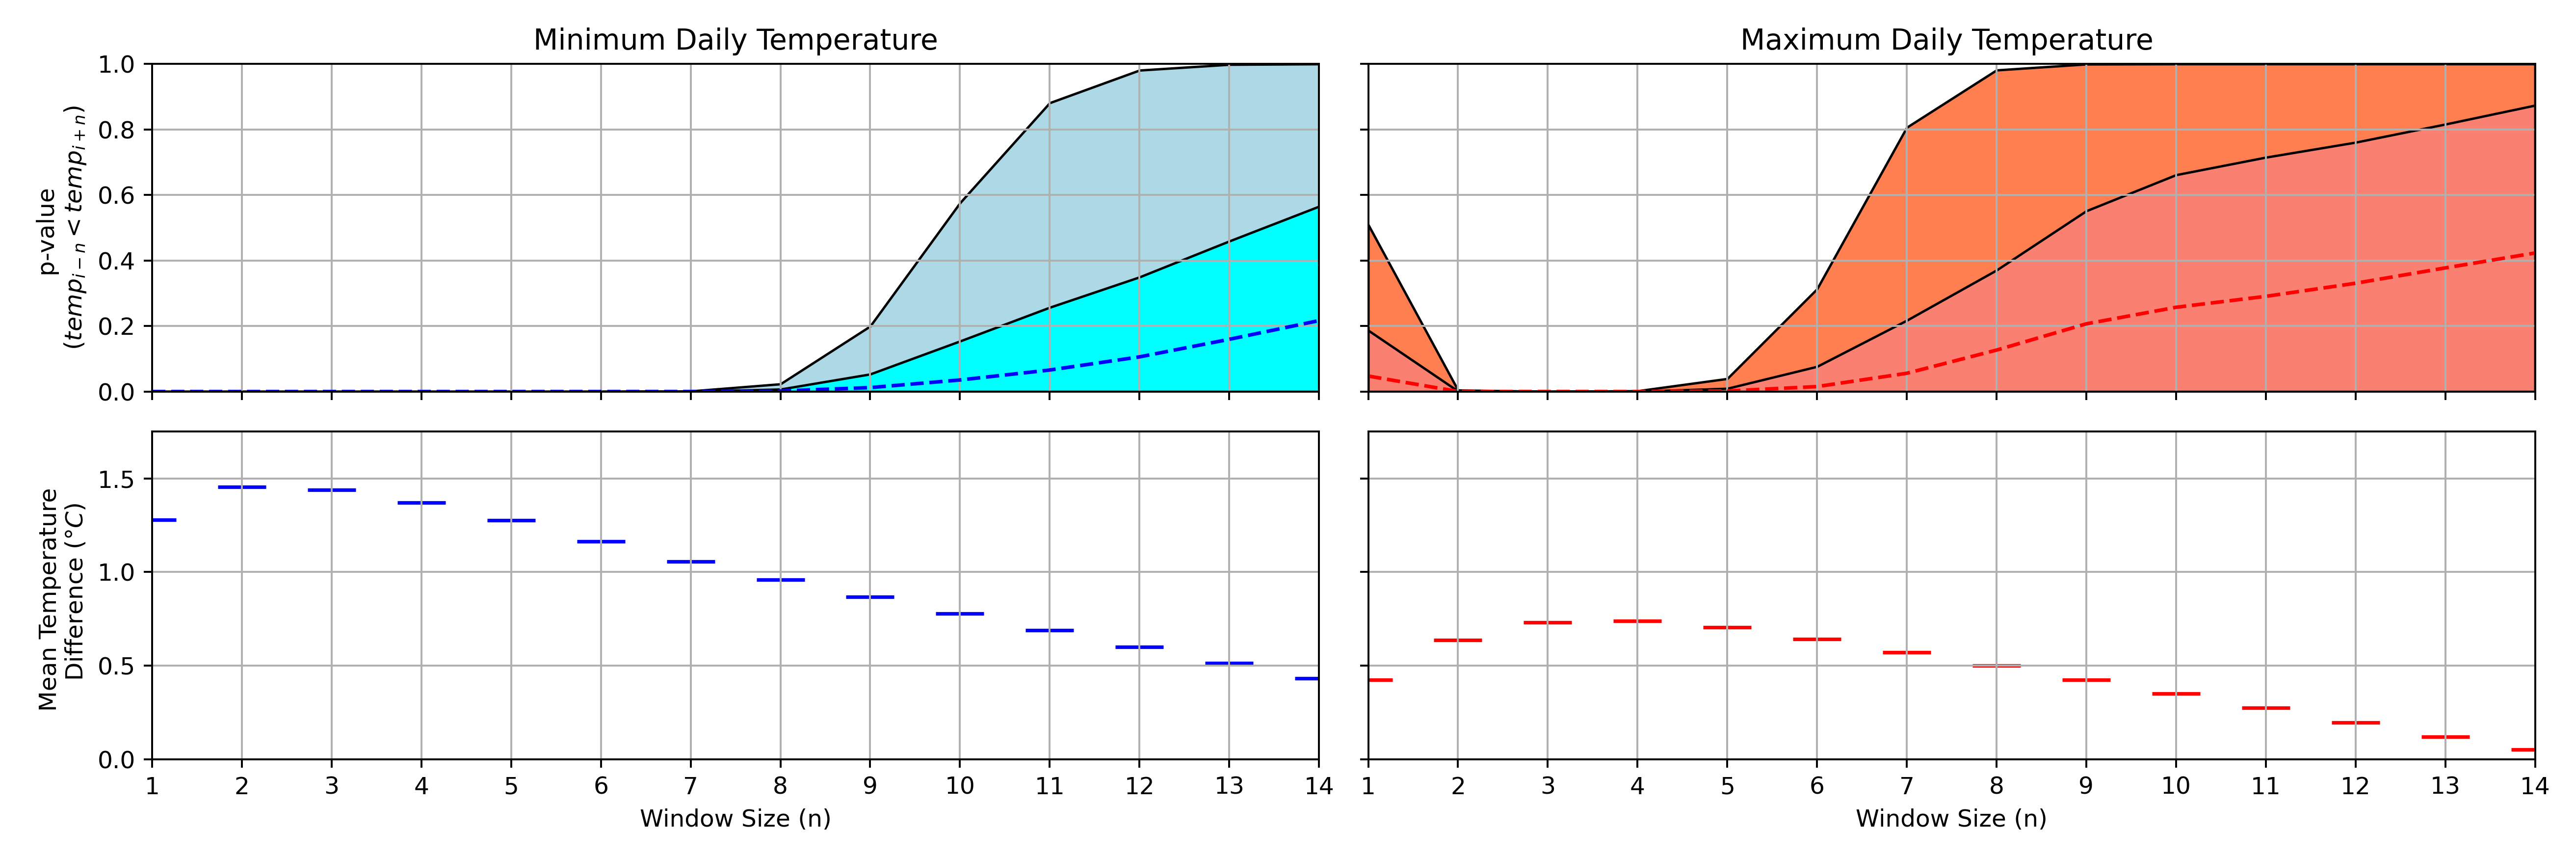
\includegraphics[width=1.0\textwidth]{./images/tmin_vs_tmax_subplots.png}
\caption{top row: the p-values of the paired t-test given the
	window size (\emph{n}) surrounding the AR event date (left:
	$T_{\text{min}}$; right: $T_{\text{max}}$). Dashed lines
	represent the mean p-value over the study area. For example, looking 
	at $T_{\text{min}}$ on the left, the light blue represents the $25^{th}$ to the 
	$75^{th}$ percentile or IQR of p-values, while the blue-grey is the $75^{th}$ 
	percentile to the maximum p-value given \emph{n}. Same is true for the 
	color transition of $T_{\text{max}}$. bottom row: the average increase
	in temperature based on AR events, calculated from the lookback 
	window to the forecast window.}
\label{fig:tmin_vs_tmax_subplots} 
\end{figure}

\subsection{AR impact on precipitation}

Figure \ref{fig:IVT_Precip_proportion_over_time} shows the AR-based IVT 
(Figure \ref{fig:IVT_Precip_proportion_over_time}A) and total precipitation 
(Figure \ref{fig:IVT_Precip_proportion_over_time}B) through the span of the 
data record,
spatially aggregated over all locations. ARs tend to account for 36\% of
precipitation on average (Figure \ref{fig:IVT_Precip_proportion_over_time}C), 
with a high degree of variability given
the year and location. In 2005 and 2020, for example, ARs accounted for nearly 
80\% of the total precipitation in some locations. Furthermore, the results 
from the Wilcoxon rank-sum test show that
precipitation from ARs tends to be greater in magnitude than non-AR 
precipitation
($\text{test statistic} = -83.85; \text{ p-value} \approx 0.0)$. In addition, it
was found that of the top 5\% of high precipitation events (HPEs), 57\% were
caused by ARs (Figure \ref{fig:concatenated_precip_var_plots}A).
Correlating annual aggregated precipitation from ARs, to total annual
aggregated precipitation in a univariate OLS, we find that the
coefficient of variation ($R^{2}$) is equal to 0.48 (Figure 
\ref{fig:concatenated_precip_var_plots}B). This indicates that ARs
explain about 48\% of interannual variability in precipitation, 
over all 25 locations.  

\begin{figure}
\centering
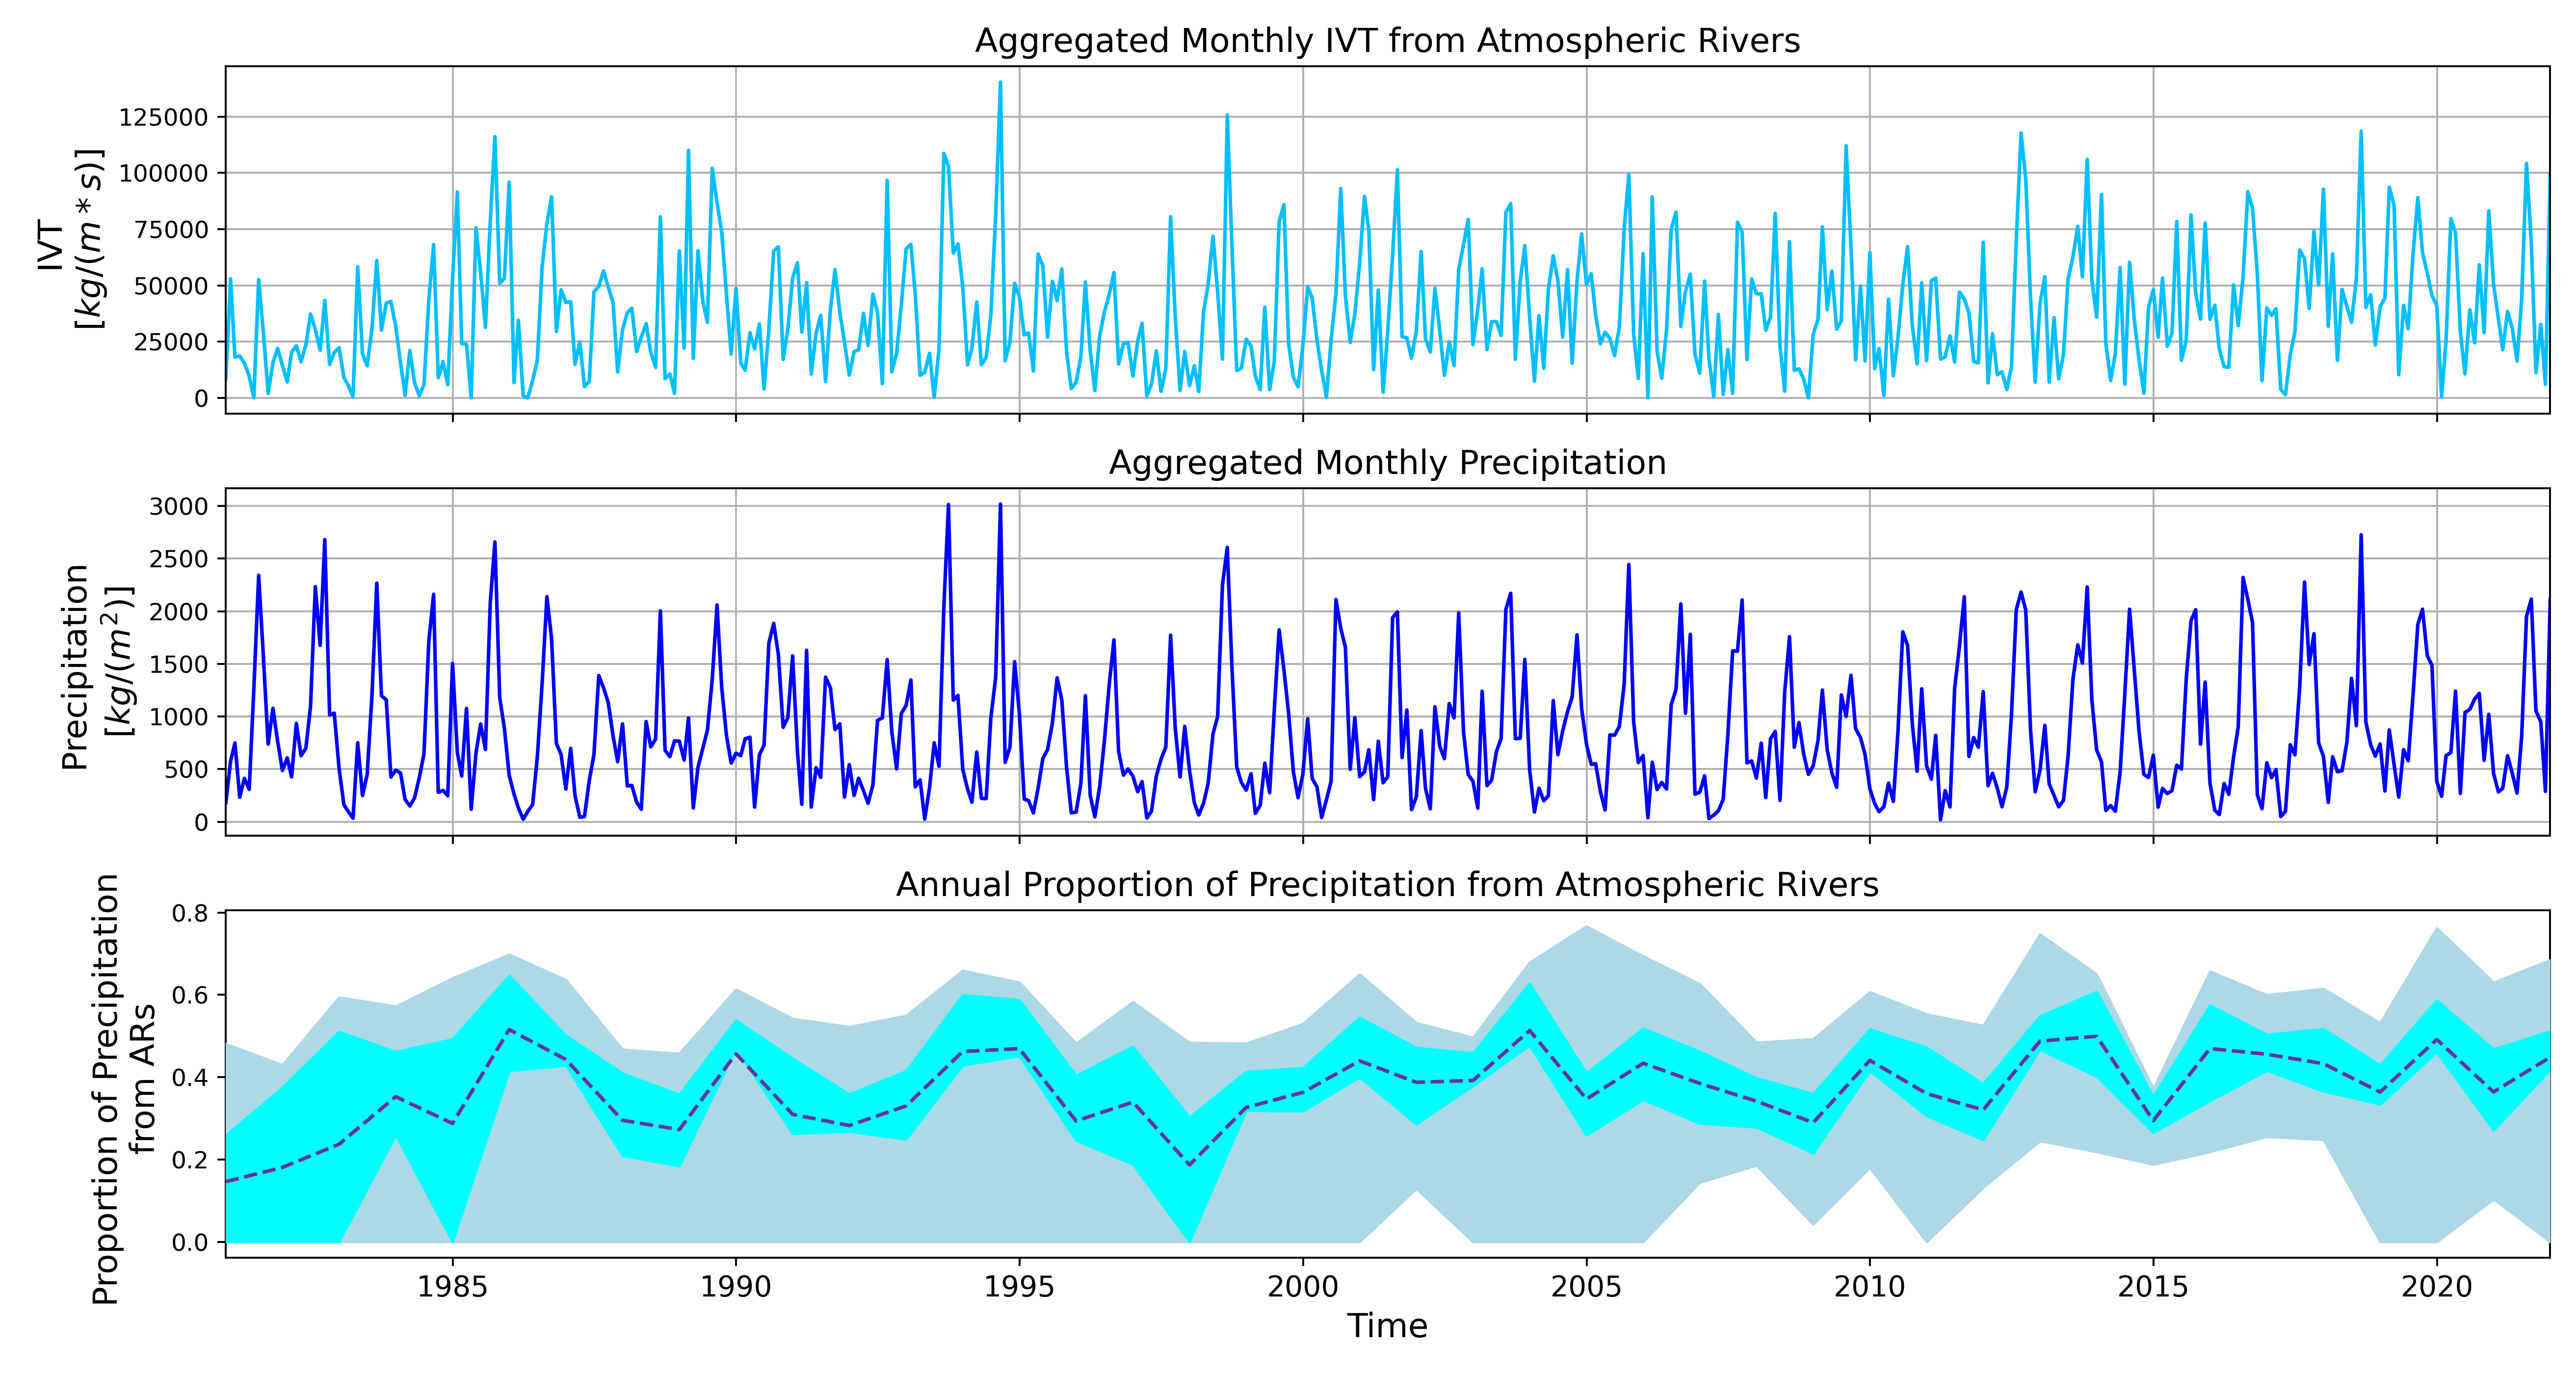
\includegraphics[width=1.0\textwidth]{./images/IVT_Precip_proportion_over_time.png}
\caption{top row: time series of IVT $\left(/frac{kg}{m*s}\right)$ aggregated monthly 
	over all locations.
	middle row: time series of total precipitation $\left(/frac{kg}{m^{2}}\right)$ 
	aggregated monthly over all
	locations. bottom row: proportion of precipitation accounted for by
	ARs on an annual basis. Light blue depicts the $25^{th}$ to $75^{th}$
	percentile (IQR) of proportion values, while the blue-grey represents 
	proportions outside of the IQR, over all 25 locations. The dashed line 
	represents the mean proportion.}
\label{fig:IVT_Precip_proportion_over_time}
\end{figure}

\subsection{Transfer of energy based on Precipitation}

To estimate the impact HPEs have on river ice breakup dates, we use 
Equation \ref{eq:final_eq} to calculate the heat transfer
between precipitation and the river ice surface. In essence, this 
exercise allows us to take the energy input from precipitation 
(whether AR-based or not) and determine whether or not that integrated 
energy accelerates or decelerates the breakup of river ice. 
We find that there is a strong negative correlation between the heat 
transfer and the DOY 
in which the river ice breaks (Figure
\ref{fig:concatenated_corr_plots}A). In this context, negative values 
along the y-axis of Figures \ref{fig:concatenated_corr_plots}A and 
\ref{fig:concatenated_corr_plots}D 
are interpreted
as a negative heat exchange, meaning a cooling effect on the river ice
surface or a deposition of precipitation below freezing. This is optimized for 
when the temporally-weighted bias curve
is positioned during the coldest period of the year - typically between
late November and early February (Figure \ref{fig:concatenated_corr_plots}C).
Table \ref{tab:pearson} shows the correlation for each location, after
tuning parameters \emph{c} and $\gamma$ are applied to Equation \ref{eq:final_eq}.
Table \ref{tab:pearson} also shows the center of the bias curve \emph{c} (month-day)
that was selected for at each location, given the integrand for precipitation used in
Equation \ref{eq:final_eq} (ie. Total Precipitation, Precipitation from ARs, Precipitation
not from ARs). 
For example, Crooked Creek on the Kuskokwim River has a
clear negative trend, with HPE causing a cooling effect on the
river ice surface, prolonging the DOY. This relationship has a Pearson correlation
coefficient $ (r_{p} )= -0.84$ and a Spearman correlation coefficient
$(r_{s}) = -0.80$, indicating that HPEs of greater magnitude, occuring 
during the coldest period of the year, lead to a delaying of the breakup date. 
The relationship between the total
number of ARs that occurred six months prior to the breakup date and the
DOY are shown in the center column 
(Figure \ref{fig:concatenated_corr_plots}B and 
\ref{fig:concatenated_corr_plots}E; 
these two plots are the same by
definition) indicating that the number of AR 
events that occur within the six months prior to the breakup
is insufficient information 
in correlating to breakup timing on its own. The
bottom row of Figure \ref{fig:concatenated_corr_plots} shows that the
use of a bias function (Equation \ref{eq:cases}) is necessary, as simply 
applying the integral of Equation \ref{eq:heat_transport} using an 
equally weighted temporal bias function (the aggregated total heat 
transfer) is uncorrelated. 


\begin{figure}
\centering
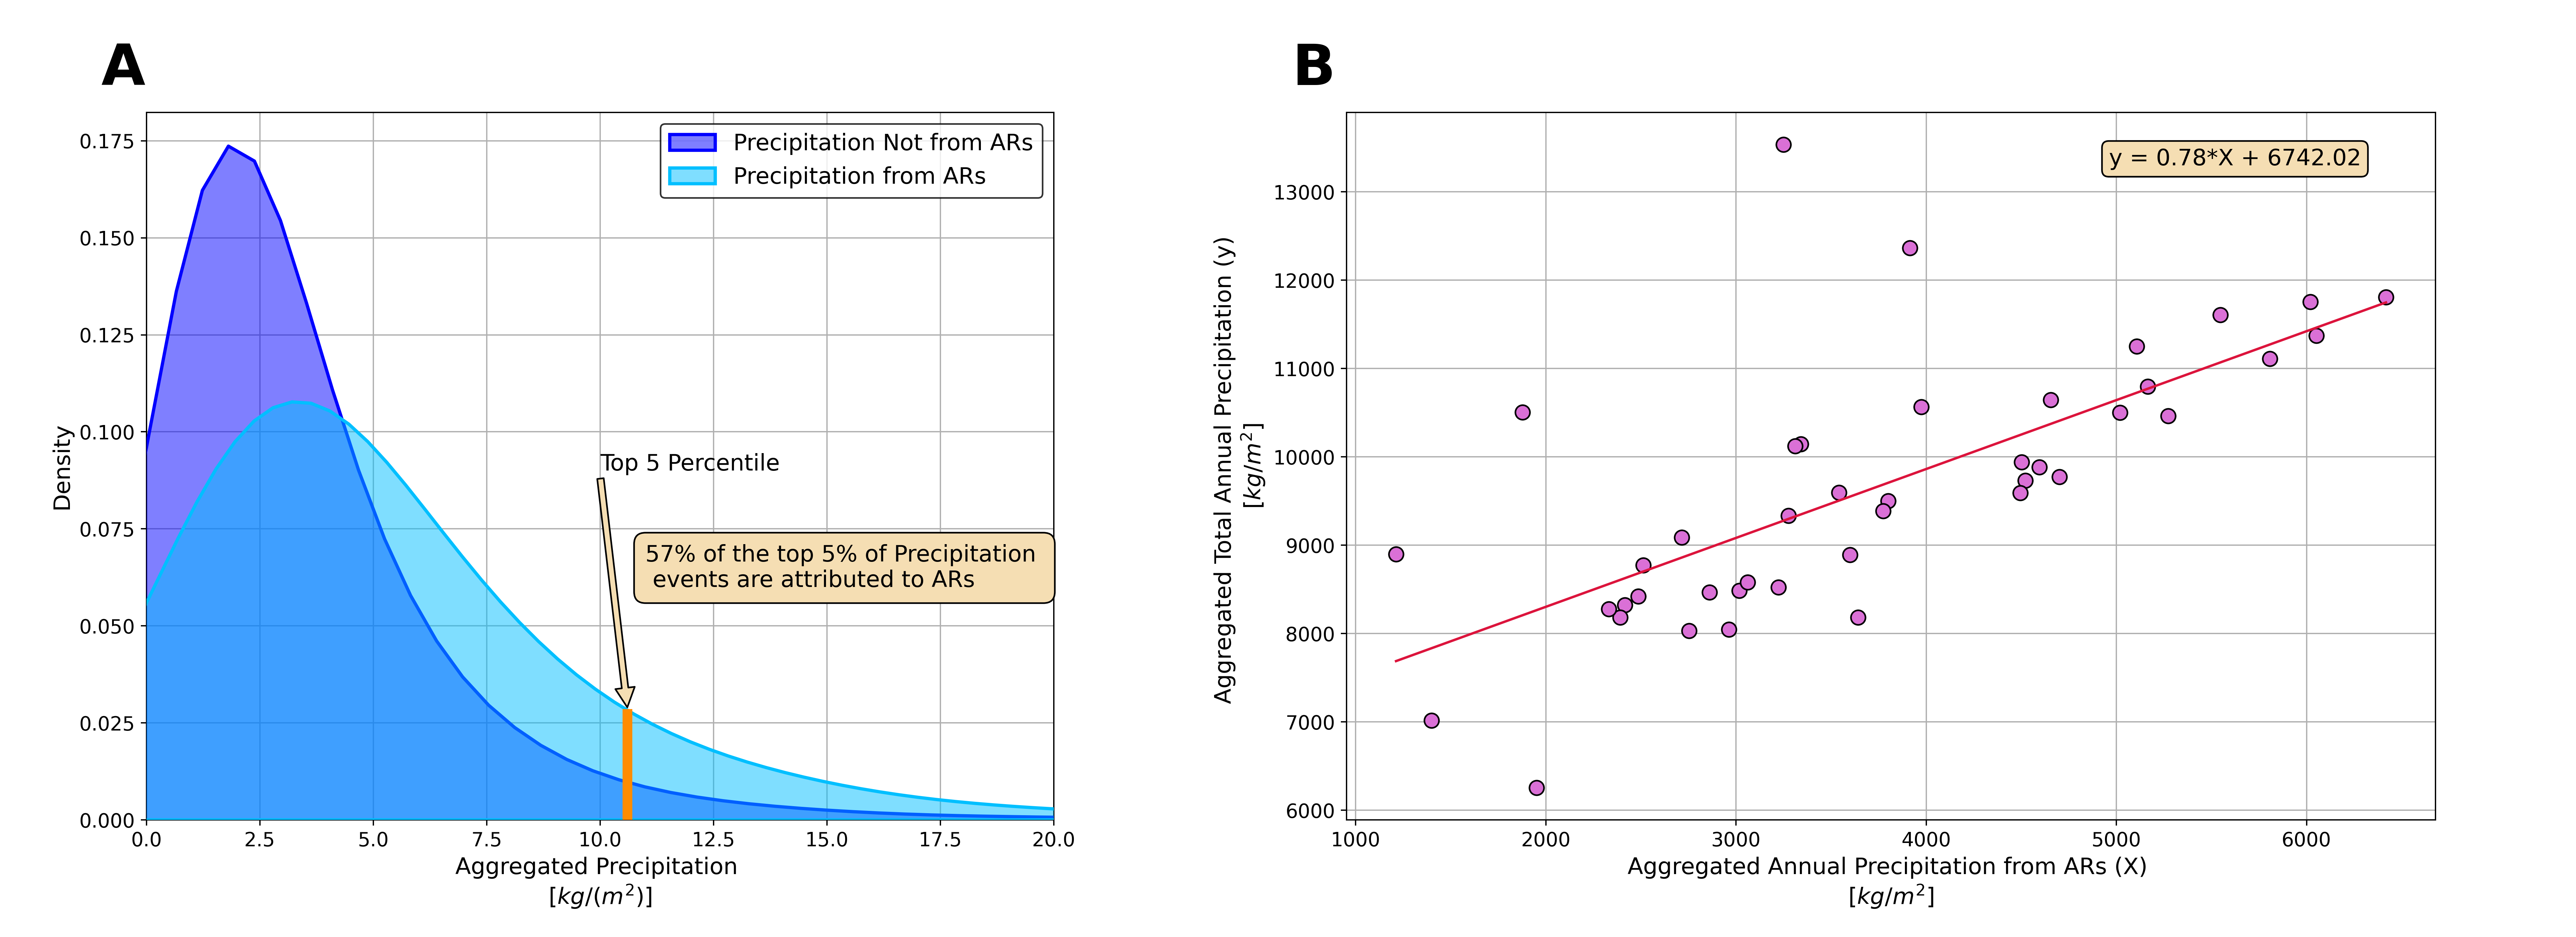
\includegraphics[width=1.0\textwidth]{./images/concatenated_precip_var_plots.png}
\caption{left: kernel density plots showing the distribution of
	local precipitation (dark blue) and precipitation from ARs
	(light blue). right: ordinary least squares regression plot
	using annual, summated precipitation from ARs, to predict total annual
	summated precipitation.}
\label{fig:concatenated_precip_var_plots}
\end{figure}

\begin{figure}[H]
\centering
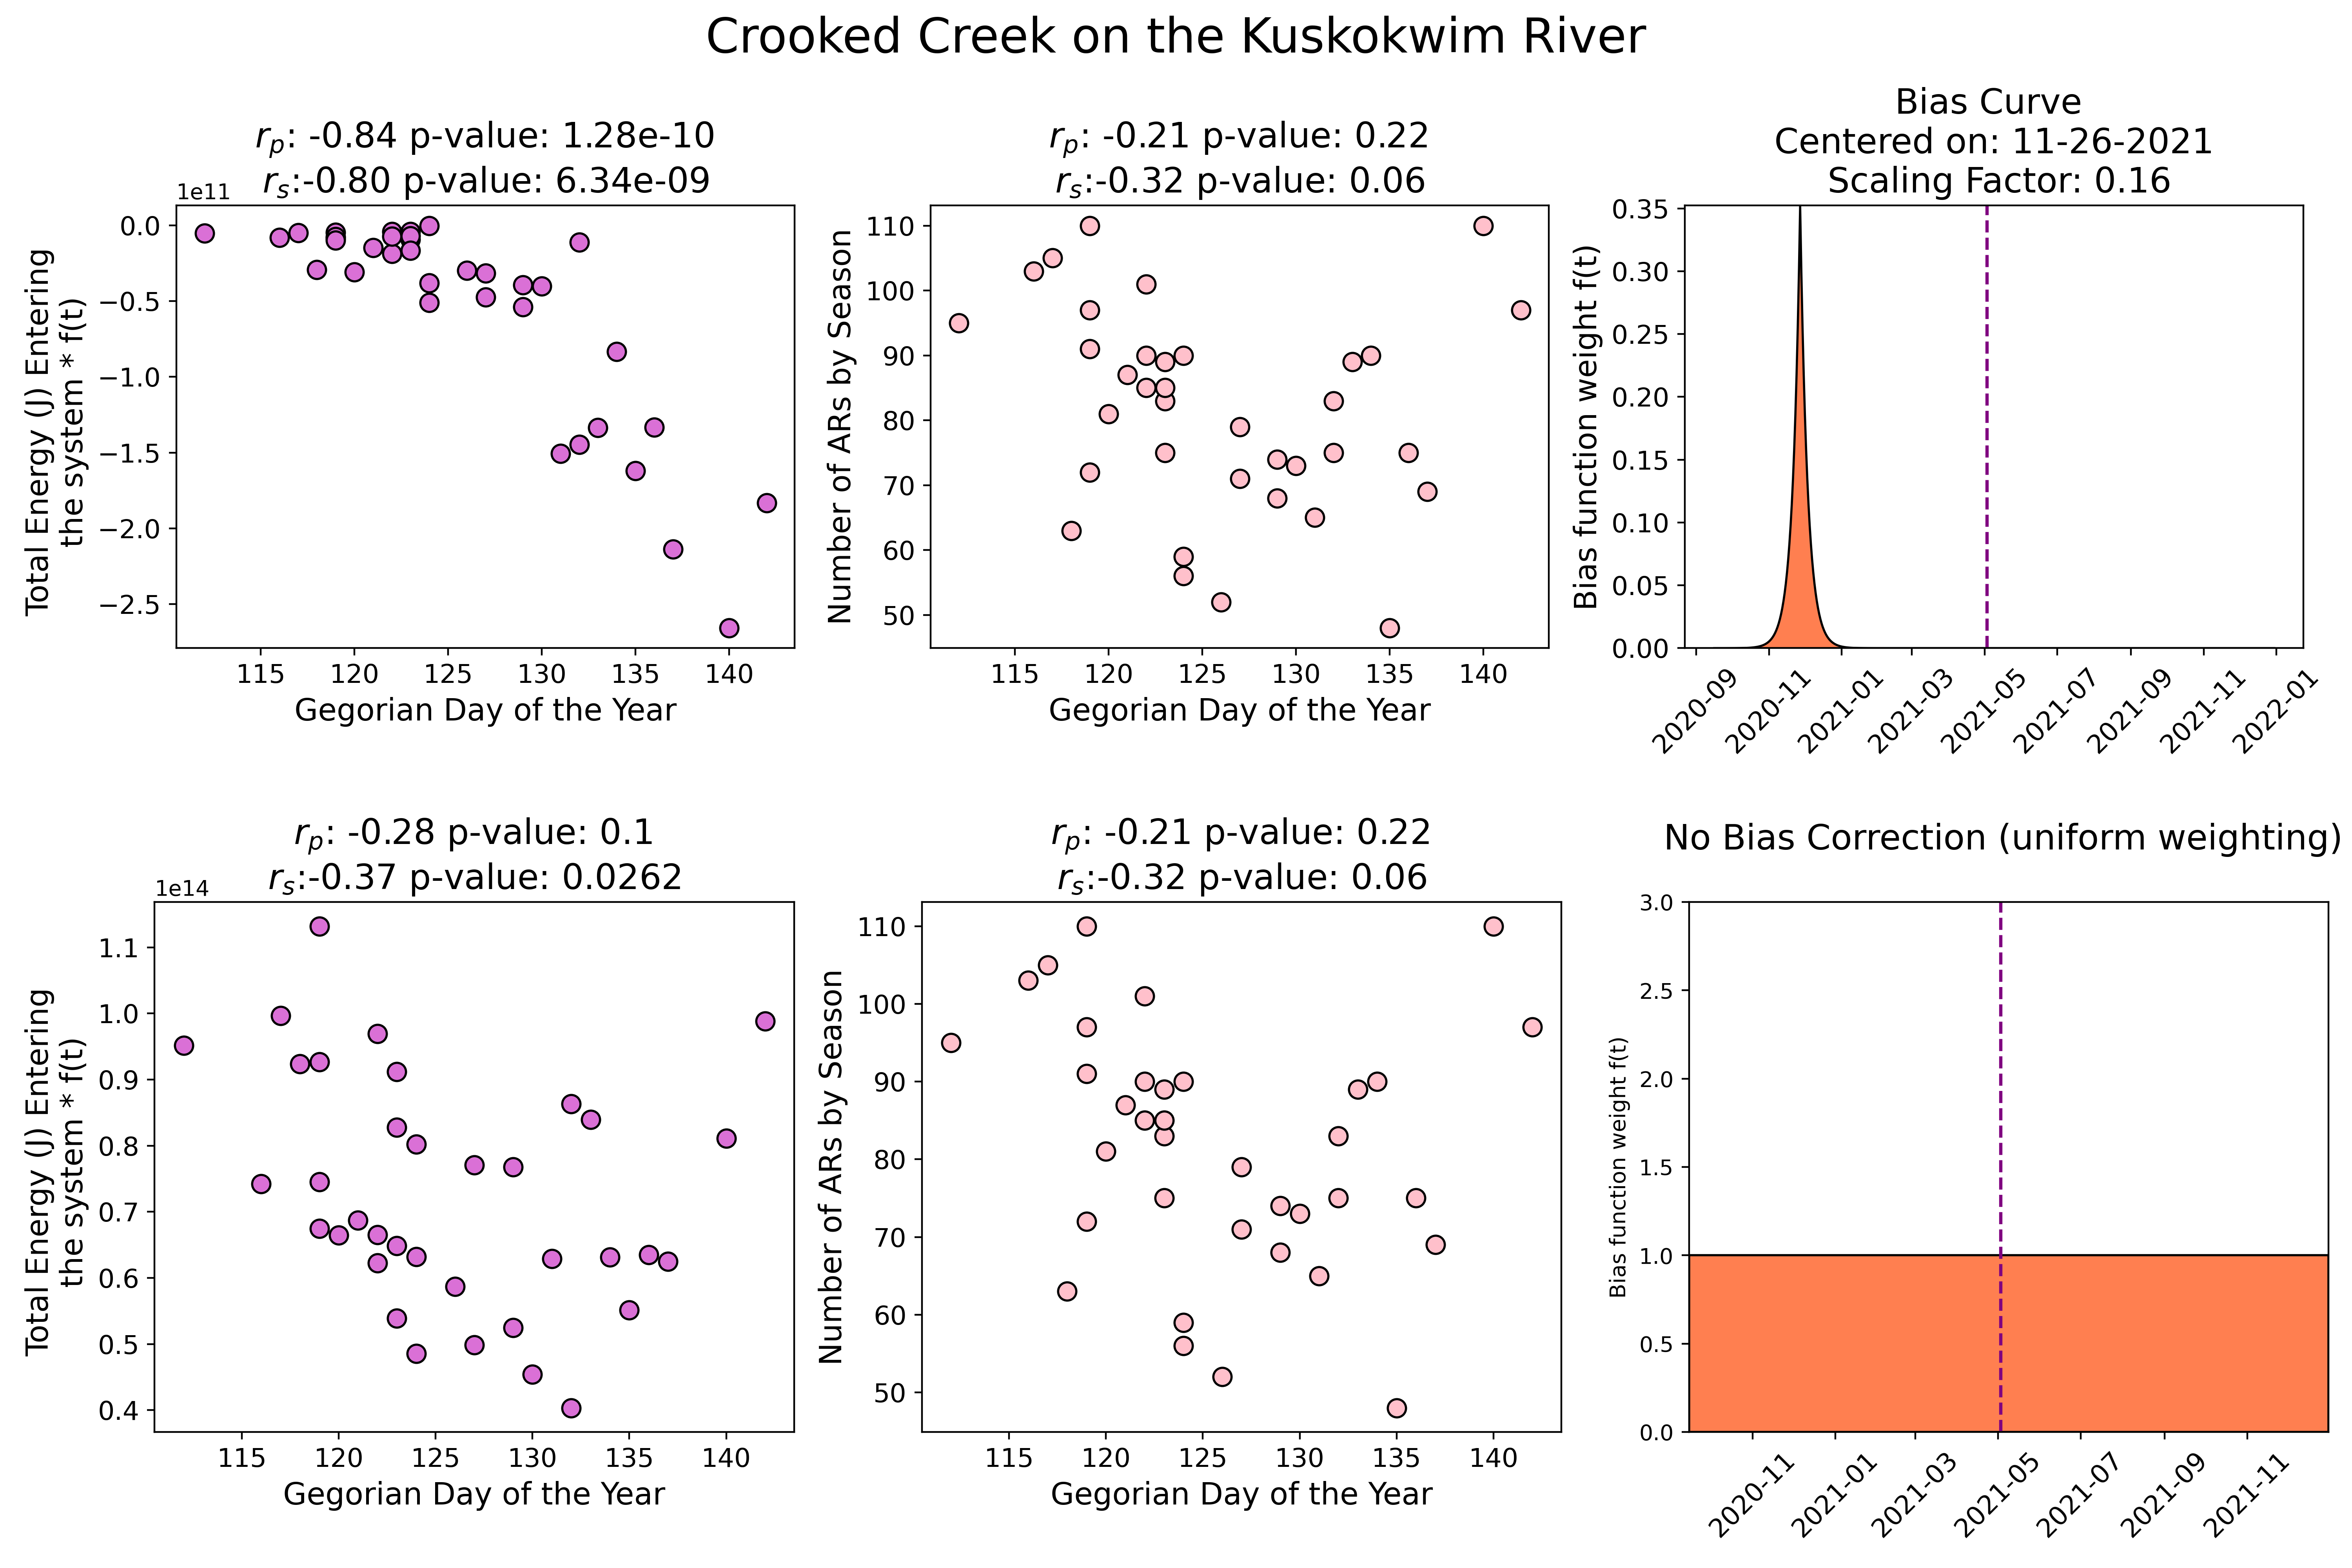
\includegraphics[width=1.0\textwidth]{./images/concatenated_scatter_bias_plots.png}
	\caption{top: (left) scatter plot between thermal energy
	transfer and DOY; (middle) scatter plot of the number of ARs
	that occured in the six months prior to the breakup date and
	DOY; 
	(right) temporal bias curve for the year 2021 with the breakup
	date represented by the vertical dashed line. bottom: same as
	the top except depicting the results when a temporal bias
	is not utilized.}
\label{fig:concatenated_corr_plots}
\end{figure}

\section{Conclusion and Discussion}

This study investigated the impact atmospheric rivers (ARs) and heavy precipitation events
(HPEs) have on the breakup dates of 
river ice in Alaska. We explored the relationship of ARs to temperature increases throughout 
the study domain, the contribution of ARs to various precipitation metrics, 
including variability and extremes, and determined the impact of ARs and HPEs on the DOY 
in which the ice on the surface of Alaskan rivers eventually breaks. 

For temperature increases, we found that ARs generally lead to a week-long persistent 
increase in daily temperature over Alaska, with temperatures rising by as much as 1.5°C 
for $T_{\text{min}}$ and 0.75°C for $T_{\text{max}}$. This result makes sense, as noted 
by many past works showing how warm moisture brought on by ARs can warm the cryosphere
\cite{Wille2021, Ma2023, ARs_lead_to_sea_ice_loss, Zhang2023}. For the contribution to 
precipitation, our results show that ARs account for a significant portion of precipitation 
in Alaska, contributing to 36\% of total precipitation on average. They also explain 48\% 
of interannual variability and make up 57\% of extreme precipitation events 
(precipitation events within the top 5\% of deposition). As for 
the relationship between ARs and river ice breakup, we show evidence that intense ARs
occurring during the coldest period of the year appear to prolong the annual breakup 
date of river ice. Our results do not show that ARs are unique relative to local forms of 
precipitation in this regard (Table \ref{tab:pearson}) with no evidence that increased 
precipitation events of any kind closer to the breakup date accelerates the breakup date.
This is likely attributed to a combination of the heat transfer from precipitation, 
as well as changes in the river ice surface as a result of snowfall. Increased snow coverage
will increase the albedo of the river surface, as well as insulate it, mitigating temperature 
fluctuations during the coldest period of the year. 

Overall, understanding the role of ARs and other HPEs in the
timing of river ice break up in Alaska is 
crucial for predicting and managing the impacts of climate change in the region, 
especially since studies have shown that AR frequency and intensity in this region are 
expected to increase in a warmer world \cite{Espinoza2018, Massoud2019}. The findings 
suggest that ARs contribute significantly to the hydrology and climate of Alaska, 
affecting temperature, precipitation, and river ice dynamics. Further research in this 
area could help improve our understanding of ARs and their role in shaping the climate 
of high-latitude regions.


%%%%%%%%%%%%%%%%%%%%%%%%%%%%%%%%%%%%%%%%%%%%%%%
%
% DATA SECTION and ACKNOWLEDGMENTS
%
%%%%%%%%%%%%%%%%%%%%%%%%%%%%%%%%%%%%%%%%%%%%%%%

\section*{Open research section}
This section MUST contain a statement that describes where the data supporting the conclusions
can be obtained. Data cannot be listed as ''Available from authors'' or stored solely in 
supporting information. Citations to archived data should be included in your reference
list. Wiley will publish it as a separate section on the paper’s page. Examples and 
complete information are here:
https://www.agu.org/Publish with AGU/Publish/Author Resources/Data for Authors


\acknowledgments
Enter acknowledgments here. This section is to acknowledge funding, thank colleagues, 
enter any secondary affiliations, and so on.


%%%%%%%%%%%%%%%%%%%%%%%%%%%%%%%%%%%%%%%%%%%%%%%
% REFERENCES and BIBLIOGRAPHY
%
% \bibliography{<name of your .bib file>} don't specify the file extension
% don't specify bibliographystyle
%
%%%%%%%%%%%%%%%%%%%%%%%%%%%%%%%%%%%%%%%%%%%%%%%

%\bibliography{ enter your bibtex bibliography filename here }
\bibliography{AR_analysis_}


%Reference citation instructions and examples:
%
% Please use ONLY \cite and \citeA for reference citations.
% \cite for parenthetical references
% ...as shown in recent studies (Simpson et al., 2019)
% \citeA for in-text citations
% ...Simpson et al. (2019) have shown...
%
%
%...as shown by \citeA{jskilby}.
%...as shown by \citeA{lewin76}, \citeA{carson86}, \citeA{bartoldy02}, and \citeA{rinaldi03}.
%...has been shown \cite{jskilbye}.
%...has been shown \cite{lewin76,carson86,bartoldy02,rinaldi03}.
%... \cite <i.e.>[]{lewin76,carson86,bartoldy02,rinaldi03}.
%...has been shown by \cite <e.g.,>[and others]{lewin76}.
%
% apacite uses < > for prenotes and [ ] for postnotes
% DO NOT use other cite commands (e.g., \citet, \citep, \citeyear, \nocite, \citealp, etc.).
%

\appendix
\section*{Appendix A.}

% Title for the table: Pearson Correlation Coefficients
\begin{table}[h]  % Place the table 'here' (h) if possible
    \centering  % Center the table
    \caption{Pearson Correlation Coefficients [$r_{p}$/Center date of bias]}  % Table caption
    \label{tab:pearson}  % Label for referencing the table
    
    % Start the tabular environment with specified column formatting
    \begin{tabular}{lccc}
    \toprule
    \textbf{Location} & \textbf{Total} & \textbf{Precipitation} & \textbf{Precipitation} \\
    \textbf{} & \textbf{Precipitation} & \textbf{from ARs} & \textbf{not from ARs} \\
    \midrule
	Akiak Kuskokwim River         &  -0.78/11-12 &    -0.78/2-5 &    -0.8/1-15 \\
	Allakaket Koyukuk River       &  -0.81/12-10 &  -0.69/10-23 &    -0.8/12-3 \\
	Ambler Kobuk River            &    -0.84/2-5 &    -0.67/2-5 &   -0.83/2-12 \\
	Aniak Kuskokwim River         &   -0.8/11-19 &   -0.81/1-29 &  -0.77/11-12 \\
	Bethel Kuskokwim River        &   -0.72/12-3 &    -0.75/2-5 &  -0.73/12-10 \\
	Bettles Koyukuk River         &   -0.79/2-19 &   -0.7/10-23 &   -0.81/2-12 \\
	Circle Yukon River            &    -0.75/2-5 &   -0.76/1-22 &   -0.74/2-12 \\
	Crooked Creek Kuskokwim River &  -0.84/11-26 &    -0.76/2-5 &   -0.8/11-26 \\
	Dawson Yukon River            &  -0.77/10-23 &   -0.67/1-22 &  -0.75/10-23 \\
	Eagle Yukon River             &  -0.77/10-23 &   -0.79/1-22 &   -0.76/1-29 \\
	Emmonak Yukon River           &    -0.76/2-5 &   -0.76/1-29 &   -0.71/4-16 \\
	Fort Yukon Yukon River        &  -0.72/10-23 &    -0.59/2-5 &  -0.72/10-23 \\
	Galena Yukon River            &  -0.79/11-19 &   -0.75/1-15 &    -0.8/4-16 \\
	Holy Cross Yukon River        &    -0.75/1-8 &    -0.77/1-8 &    -0.72/1-8 \\
	Hughes Koyukuk River          &    -0.81/1-1 &   -0.78/1-15 &    -0.78/4-2 \\
	Kaltag Yukon River            &   -0.84/12-3 &   -0.77/12-3 &   -0.86/1-15 \\
	Kobuk Kobuk River             &    -0.81/1-8 &   -0.62/4-16 &    -0.81/1-8 \\
	McGrath Kuskokwim River       &   -0.81/3-26 &    -0.81/2-5 &    -0.82/4-9 \\
	Mountain Village Yukon River  &   -0.72/1-29 &    -0.76/2-5 &   -0.69/2-19 \\
	Nenana Tanana River           &    -0.71/1-1 &    -0.73/2-5 &    -0.72/1-1 \\
	Nikolai Kuskokwim River       &   -0.75/2-12 &     -0.7/2-5 &   -0.74/1-15 \\
	Red Devil Kuskokwim River     &   -0.79/12-3 &     -0.8/2-5 &   -0.78/12-3 \\
	Ruby Yukon River              &    -0.83/4-9 &   -0.78/1-15 &   -0.86/4-16 \\
	Russian Mission Yukon River   &  -0.71/11-26 &  -0.72/12-10 &   -0.68/12-3 \\
	Tanana Yukon River            &   -0.76/1-22 &     -0.7/2-5 &  -0.77/11-26 \\
    \bottomrule
    \end{tabular}
\end{table}


\end{document}






































% More Information and Advice:

%%

%  Numbered lines in equations:
%  To add line numbers to lines in equations,
%  \begin{linenomath*}
%  \begin{equation}
%  \end{equation}
%  \end{linenomath*}



%% Enter Figures and Tables near as possible to where they are first mentioned:
%
% DO NOT USE \psfrag or \subfigure commands.
%
% Figure captions go below the figure.
% Acronyms used in figure captions will be spelled out in the final, published version.

% Table titles go above tables;  other caption information
%  should be placed in last line of the table, using
% \multicolumn2l{$^a$ This is a table note.}
% NOTE that there is no difference between table caption and table heading in the final, published version
%
%----------------
% EXAMPLE FIGURES
%
% \begin{figure}
% \includegraphics{example.png}
% \caption{caption}
% \end{figure}
%
% Giving latex a width will help it to scale the figure properly. A simple trick is to use 
% \textwidth. Try this if large figures run off the side of the page.
% \begin{figure}
% \noindent\includegraphics[width=\textwidth]{anothersample.png}
%\caption{caption}
%\label{pngfiguresample}
%\end{figure}
%
%
% If you get an error about an unknown bounding box, try specifying the width and height 
% of the figure with the natwidth and natheight options. This is common when trying to add a PDF figure without pdflatex.
% \begin{figure}
% \noindent\includegraphics[natwidth=800px,natheight=600px]{samplefigure.pdf}
%\caption{caption}
%\label{pdffiguresample}
%\end{figure}
%
%
% PDFLatex does not seem to be able to process EPS figures. You may want to try the epstopdf package.
%

%
% ---------------
% EXAMPLE TABLE
%
% \begin{table}
% \caption{Time of the Transition Between Phase 1 and Phase 2$^{a}$}
% \centering
% \begin{tabular}{l c}
% \hline
%  Run  & Time (min)  \\
% \hline
%   $l1$  & 260   \\
%   $l2$  & 300   \\
%   $l3$  & 340   \\
%   $h1$  & 270   \\
%   $h2$  & 250   \\
%   $h3$  & 380   \\
%   $r1$  & 370   \\
%   $r2$  & 390   \\
% \hline
% \multicolumn{2}{l}{$^{a}$Footnote text here.}
% \end{tabular}
% \end{table}

%%%%%%%%%%%%%%%%%%%%%%%%%%%%%%%%%%%%%%%%%%%%%%%
% SIDEWAYS FIGURES and TABLES
% AGU prefers the use of {sidewaystable} over {landscapetable} as it causes fewer problems.
%
% \begin{sidewaysfigure}
% \includegraphics[width=20pc]{figsamp}
% \caption{caption here}
% \label{newfig}
% \end{sidewaysfigure}
%
%  \begin{sidewaystable}
%  \caption{Caption here}
% \label{tab:signif_gap_clos}
%  \begin{tabular}{ccc}
% one&two&three\\
% four&five&six
%  \end{tabular}
%  \end{sidewaystable}

%% If using numbered lines, please surround equations with \begin{linenomath*}...\end{linenomath*}
%\begin{linenomath*}
%\begin{equation}
%y|{f} \sim g(m, \sigma),
%\end{equation}
%\end{linenomath*}

%%% End of body of article

%%%%%%%%%%%%%%%%%%%%%%%%%%%%%%%%%%%%%%%%%%%%%%%
%% Optional Appendices go here
%
% The \appendix command resets counters and redefines section heads
%
% After typing \appendix
%
%\section{Here Is Appendix Title}
% will show
% A: Here Is Appendix Title
%

%%%%%%%%%%%%%%%%%%%%%%%%%%%%%%%%%%%%%%%%%%%%%%%
% Optional Glossary, Notation or Acronym section goes here:
%
% Glossary is only allowed in Reviews of Geophysics
%  \begin{glossary}
%  \term{Term}
%   Term Definition here
%  \term{Term}
%   Term Definition here
%  \term{Term}
%   Term Definition here
%  \end{glossary}


%%%%%%%%%%%%%%%%%%%%%%%%%%%%%%%%%%%%%%%%%%%%%%%
% Acronyms
%% NOTE that acronyms in the final published version will be spelled out when used in figure captions.
%   \begin{acronyms}
%   \acro{Acronym}
%   Definition here
%   \acro{EMOS}
%   Ensemble model output statistics
%   \acro{ECMWF}
%   Centre for Medium-Range Weather Forecasts
%   \end{acronyms}


%%%%%%%%%%%%%%%%%%%%%%%%%%%%%%%%%%%%%%%%%%%%%%%
% Notation
%   \begin{notation}
%   \notation{$a+b$} Notation Definition here
%   \notation{$e=mc^2$}
%   Equation in German-born physicist Albert Einstein's theory of special
%  relativity that showed that the increased relativistic mass ($m$) of a
%  body comes from the energy of motion of the body—that is, its kinetic
%  energy ($E$)—divided by the speed of light squared ($c^2$).
%   \end{notation}


%%%%%%%%%%%%%%%%%%%%%%%%%%%%%%%%%%%%%%%%%%%%%%%
%
%  SECTION HEADS
%
%%%%%%%%%%%%%%%%%%%%%%%%%%%%%%%%%%%%%%%%%%%%%%%

% Capitalize the first letter of each word (except for
% prepositions, conjunctions, and articles that are
% three or fewer letters).

% AGU follows standard outline style; therefore, there cannot be a section 1 without
% a section 2, or a section 2.3.1 without a section 2.3.2.
% Please make sure your section numbers are balanced.
% ---------------
% Level 1 head
%
% Use the \section{} command to identify level 1 heads;
% type the appropriate head wording between the curly
% brackets, as shown below.
%
%An example:
%\section{Level 1 Head: Introduction}
%
% ---------------
% Level 2 head
%
% Use the \subsection{} command to identify level 2 heads.
%An example:
%\subsection{Level 2 Head}
%
% ---------------
% Level 3 head
%
% Use the \subsubsection{} command to identify level 3 heads
%An example:
%\subsubsection{Level 3 Head}
%
%---------------
% Level 4 head
%
% Use the \subsubsubsection{} command to identify level 3 heads
% An example:
%\subsubsubsection{Level 4 Head} An example.
%
%%%%%%%%%%%%%%%%%%%%%%%%%%%%%%%%%%%%%%%%%%%%%%%
%
%  IN-TEXT LISTS
%
%%%%%%%%%%%%%%%%%%%%%%%%%%%%%%%%%%%%%%%%%%%%%%%
%
% Do not use bulleted lists; enumerated lists are okay.
% \begin{enumerate}
% \item
% \item
% \item
% \end{enumerate}
%
%%%%%%%%%%%%%%%%%%%%%%%%%%%%%%%%%%%%%%%%%%%%%%%
%
%  EQUATIONS
%
%%%%%%%%%%%%%%%%%%%%%%%%%%%%%%%%%%%%%%%%%%%%%%%

% Single-line equations are centered.
% Equation arrays will appear left-aligned.

%Math coded inside display math mode \[ ...\]
% will not be numbered, e.g.,:
% \[ x^2=y^2 + z^2\]

% Math coded inside \begin{equation} and %\end{equation} will
% be automatically numbered, e.g.,:
% \begin{equation}
% x^2=y^2 + z^2
% \end{equation}


% To create multiline equations, use the
% \begin{eqnarray} and \end{eqnarray} environment
% as demonstrated below.
%\begin{eqnarray}
 % x_{1} & = & (x - x_{0}) \cos \Theta \nonumber \\
 %       && + (y - y_{0}) \sin \Theta  \nonumber \\
%  y_{1} & = & -(x - x_{0}) \sin \Theta \nonumber \\
 %       && + (y - y_{0}) \cos \Theta.
%\end{eqnarray}

%If you don't want an equation number, use the star form:
%\begin{eqnarray*}...\end{eqnarray*}

% Break each line at a sign of operation
% (+, -, etc.) if possible, with the sign of operation
% on the new line.

% Indent second and subsequent lines to align with
% the first character following the equal sign on the
% first line.

% Use an \hspace{} command to insert horizontal space
% into your equation if necessary. Place an appropriate
% unit of measure between the curly braces, e.g.
% \hspace{1in}; you may have to experiment to achieve
% the correct amount of space.


%%%%%%%%%%%%%%%%%%%%%%%%%%%%%%%%%%%%%%%%%%%%%%%
%
%  EQUATION NUMBERING: COUNTER
%
%%%%%%%%%%%%%%%%%%%%%%%%%%%%%%%%%%%%%%%%%%%%%%%

% You may change equation numbering by resetting
% the equation counter or by explicitly numbering
% an equation.

% To explicitly number an equation, type \eqnum{}
% (with the desired number between the brackets)
% after the \begin{equation} or \begin{eqnarray}
% command.  The \eqnum{} command will affect only
% the equation it appears with; LaTeX will number
% any equations appearing later in the manuscript
% according to the equation counter.
%

% If you have a multiline equation that needs only
% one equation number, use a \nonumber command in
% front of the double backslashes (\\) as shown in
% the multiline equation above.

% If you are using line numbers, remember to surround
% equations with \begin{linenomath*}...\end{linenomath*}

%  To add line numbers to lines in equations:
%  \begin{linenomath*}
%  \begin{equation}
%  \end{equation}
%  \end{linenomath*}




